\chapter{尺规作图}
\begin{problem}[怀新一题 | 双曲测地线]
    给定欧几里得平面上的一个圆 $C_1$ 和两个不同的点 $A$,$B$。假设过 $A$,$B$ 的直线不经过 $C_1$ 的圆心。
    用直尺(没有刻度)和圆规作出一个过 $A$,$B$ 的圆 $C_2$,使得 $C_1$ 和 $C_2$交于两个点 $P$,$Q$,并且在交点 $P$,$Q$ 处垂直。
    注意 $A$,$B$ 分别可以在 $C_1$ 内,$C_1$ 外或 $C_1$ 上。
\end{problem}
\begin{proof}
    分析题目, 我们知道双曲平面有几种经典模型, 其中两种是 Poicar\'e 圆盘模型和上半平面模型. 在圆盘模型中, 过单位圆内两点的测地线经过延长后与边界正交, 所以要么是直径,
    要么就是题目所求的圆 $C_2$ 的一部分.
    \begin{figure}[htbp]
        \centering
        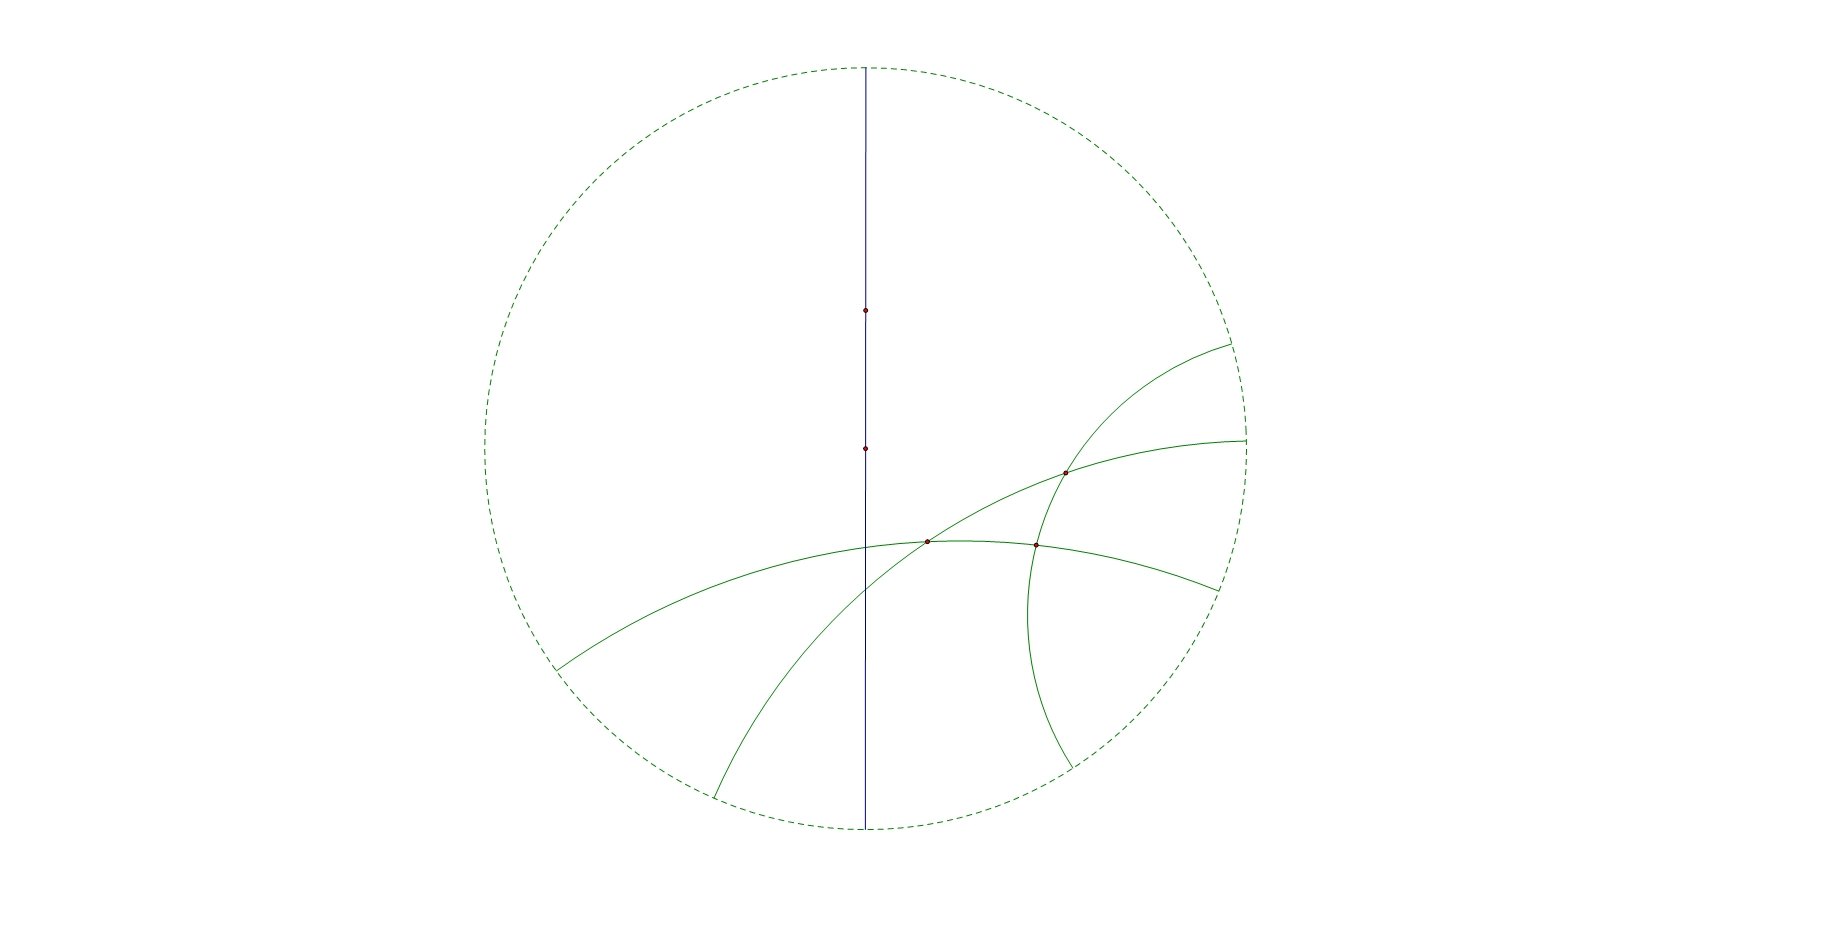
\includegraphics[scale = 0.18]{Figures/geo-in-D2.png}
        \caption{Poincar\'e 圆盘模型中的测地线}
    \end{figure}

    在上半平面模型中过两点的测地线经延长后要么是与横轴垂直的射线, 要么是与横轴正交的上半圆. 
    \begin{figure}[htbp]
        \centering
        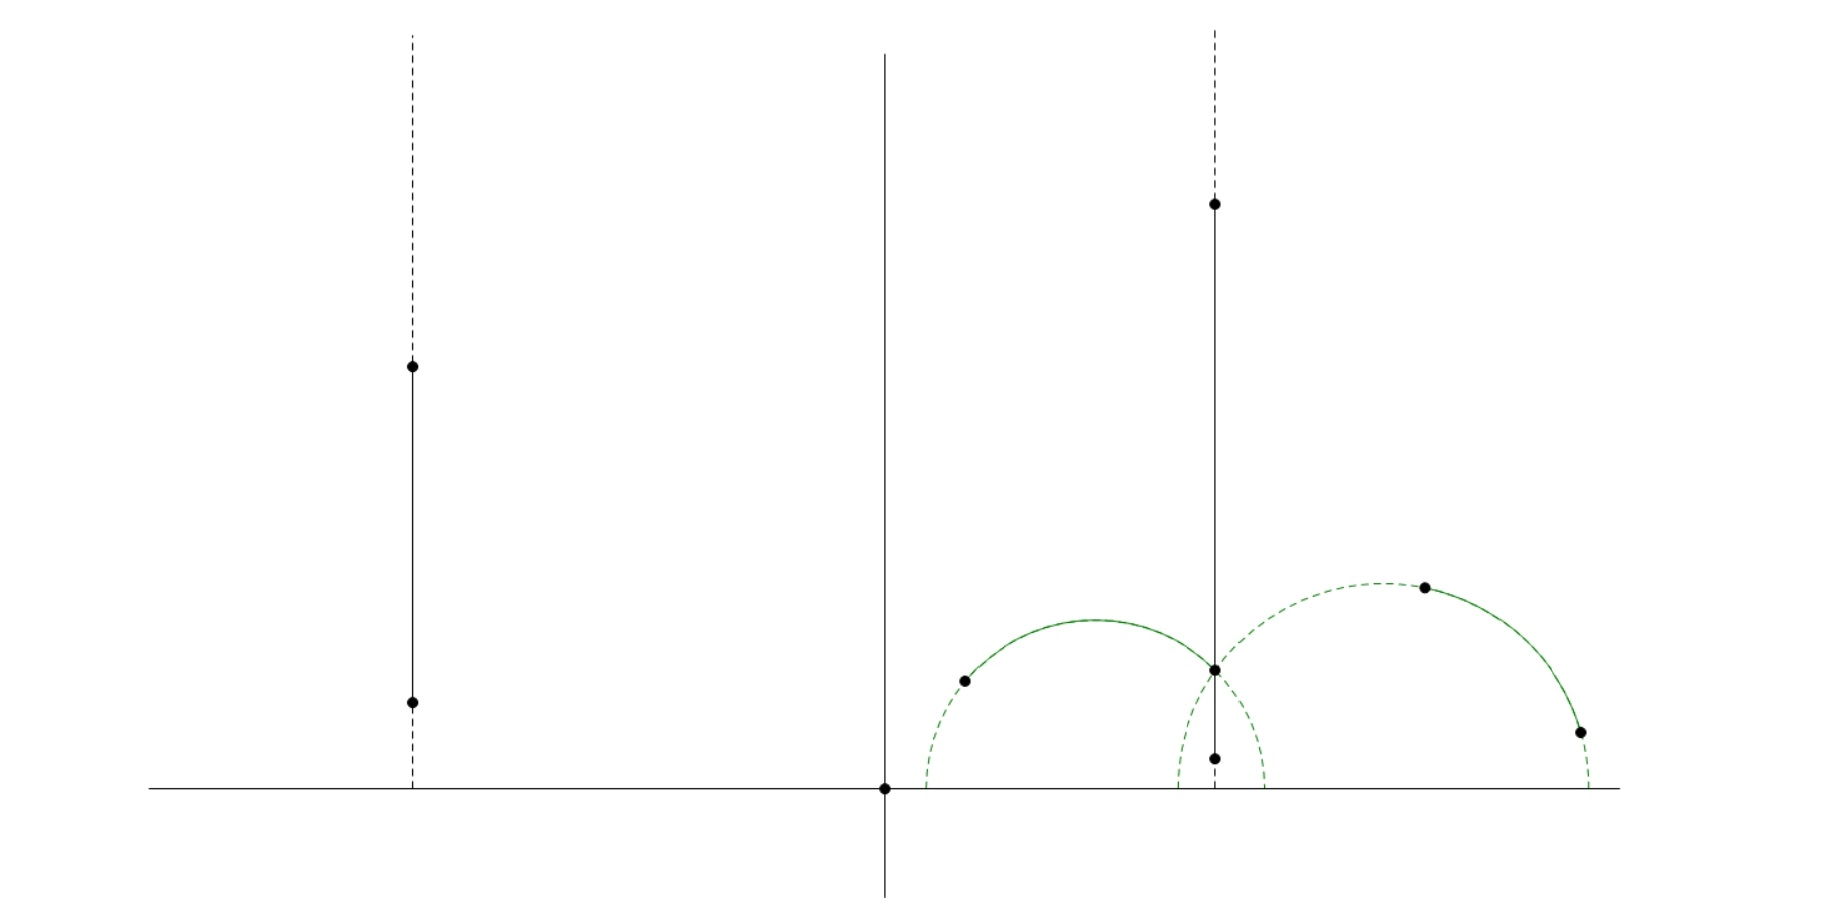
\includegraphics[scale = 0.2]{Figures/geo-in-H2.png}
        \caption{上半平面模型中的测地线}
    \end{figure}

    同时两个模型之间也有相互转化的关系, 用坐标表达就是 Cayley 变换, 用平面几何的语言就是反演变换. 于是我们可以用反演变换将原问题转化为:

    给定一条直线 $l$ 以及两点 $A'$, $B'$. 假设过 $A'$, $B'$ 的直线不与 $l$ 垂直, 用尺规作出一个过 $A'$,$B'$ 的圆 $C_2'$, 使得 $l$ 和 $C_2$交于两个点 $P'$,$Q'$, 并且在交点 $P'$,$Q'$ 处垂直. 
    
    注意到最后一个垂直条件实际上等价于圆心 $C_2'$ 在直线 $l$ 上, 于是我们把原来复杂的问题转化为一个简单的尺规作图问题.

    下面开始陈述作图过程, 简便起见我们略去一些基础尺规作图的过程.
    \begin{enumerate}
        \item 在圆 $C_1$ 上任取一点 $X$, 以 $D$ 为圆心作圆 $X$ 使其与圆 $C_1$ 交于两点 $E$, $F$. 连接 $E$, $F$ 得到直线 $l$, 此即圆 $C_1$ 关于圆 $D$ 反演后的图形.
        \item 连接线段 $DA$, 取其中点 $M$, 以 $M$ 为圆心, $MD$ 为半径作圆 $M$. 设圆 $M$ 交圆 $D$ 于两点 $G$, $H$, 连接线段 $GH$ 交线段 $AD$ 于点 $A'$, 此即点 $A$ 关于圆 $D$ 反演后的图形. 
        \item 同理可作点 $B$ 关于圆 $D$ 反演后的点 $B'$.
        \item 作线段 $A'B'$ 的中垂线, 交直线 $l$ 于点 $C_2'$, 由题目条件可知 $A'B'$ 不可能与 $l$ 垂直, 因此交点 $C_2'$ 一定存在.
        \item 类似地作出 $C_2'$ 关于圆 $D$ 反演后的点 $C_2$, 以 $C_2$ 为圆心, $CA$ 为半径作圆, 此即所求.
    \end{enumerate}
    \begin{figure}[htbp]
        \centering
        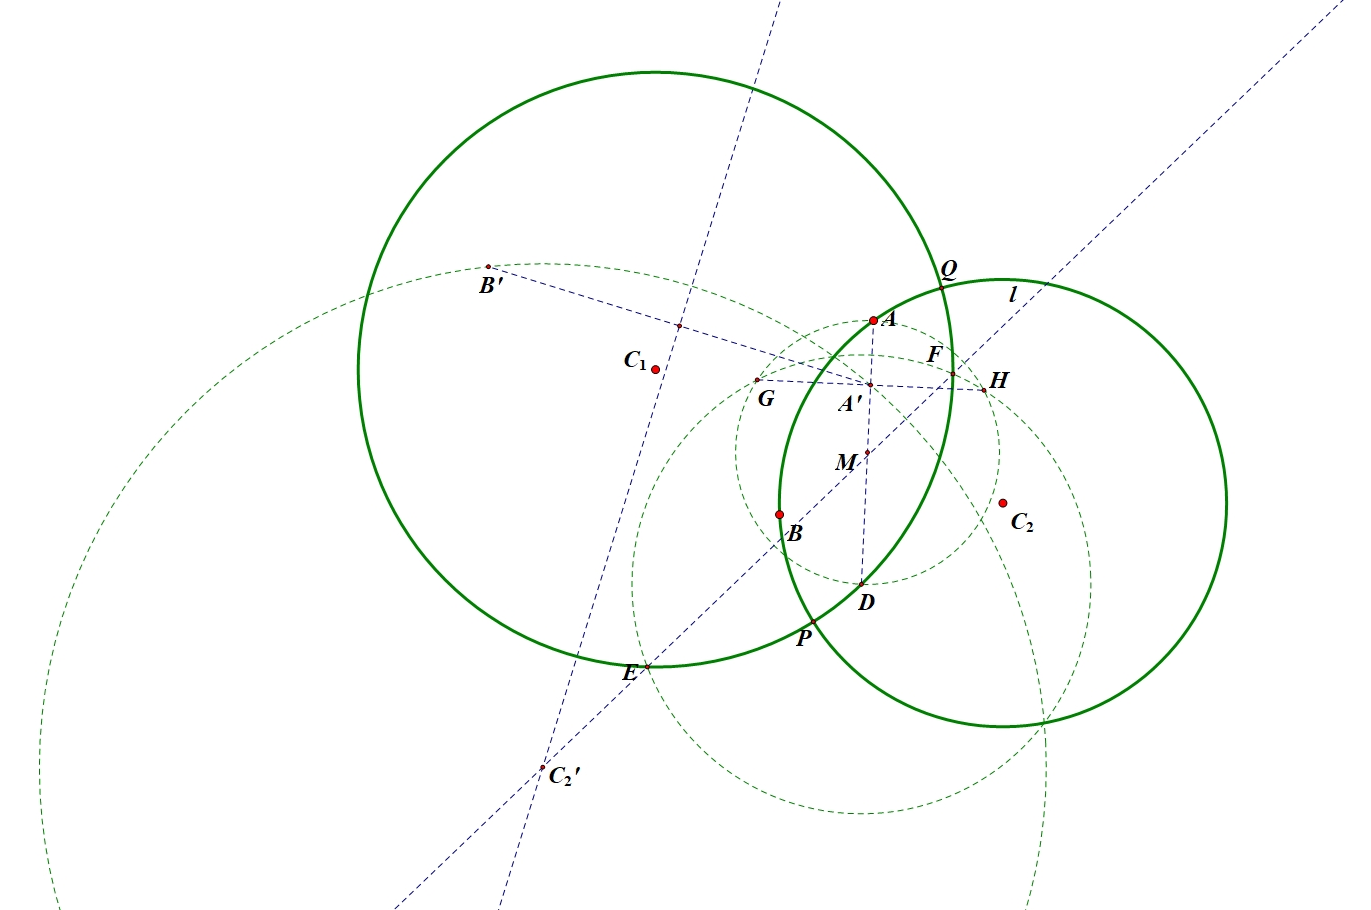
\includegraphics[scale = 0.4]{Figures/怀新一题(1).png}
    \end{figure}
\end{proof}
\begin{remark}
    此做法与点 $A$, $B$ 和圆 $C_1$ 的位置关系无关, 例如下面几种位置关系:
    \begin{figure}[htbp]
        \centering
        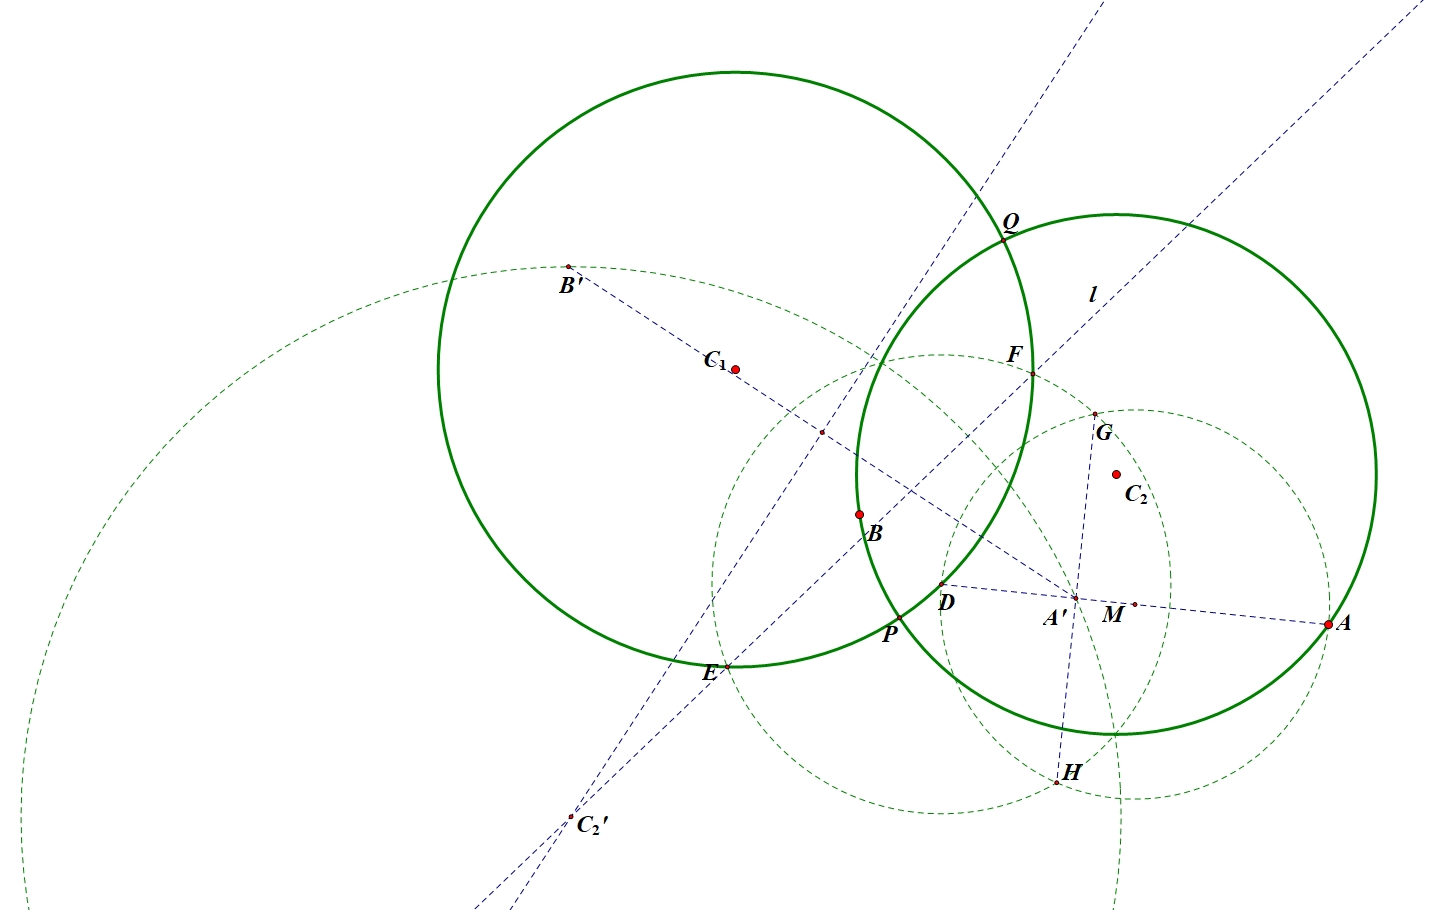
\includegraphics[scale = 0.31]{Figures/怀新一题(2).png}
        \caption{点 $A$ 在圆外, 点 $B$ 在圆内}                 
    \end{figure}
    \begin{figure}[htbp]
        \centering
        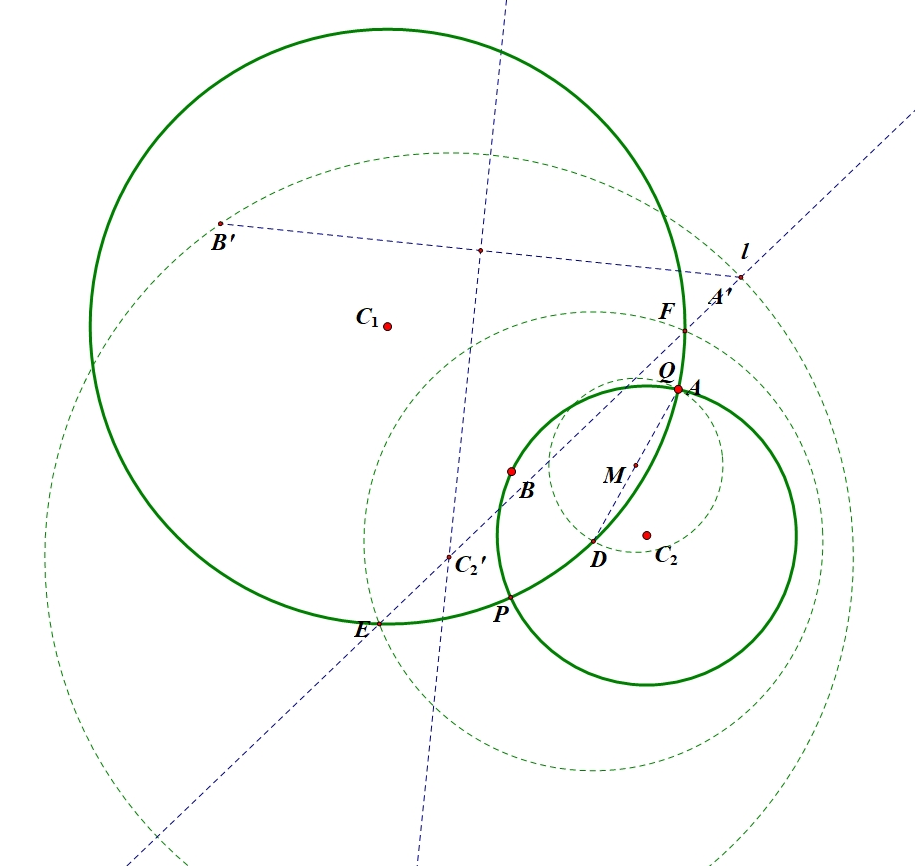
\includegraphics[scale = 0.31]{Figures/怀新一题(3).png}
        \caption{点 $A$ 在圆上, 点 $B$ 在圆内}
    \end{figure}
    \begin{figure}[htbp]
        \centering            
        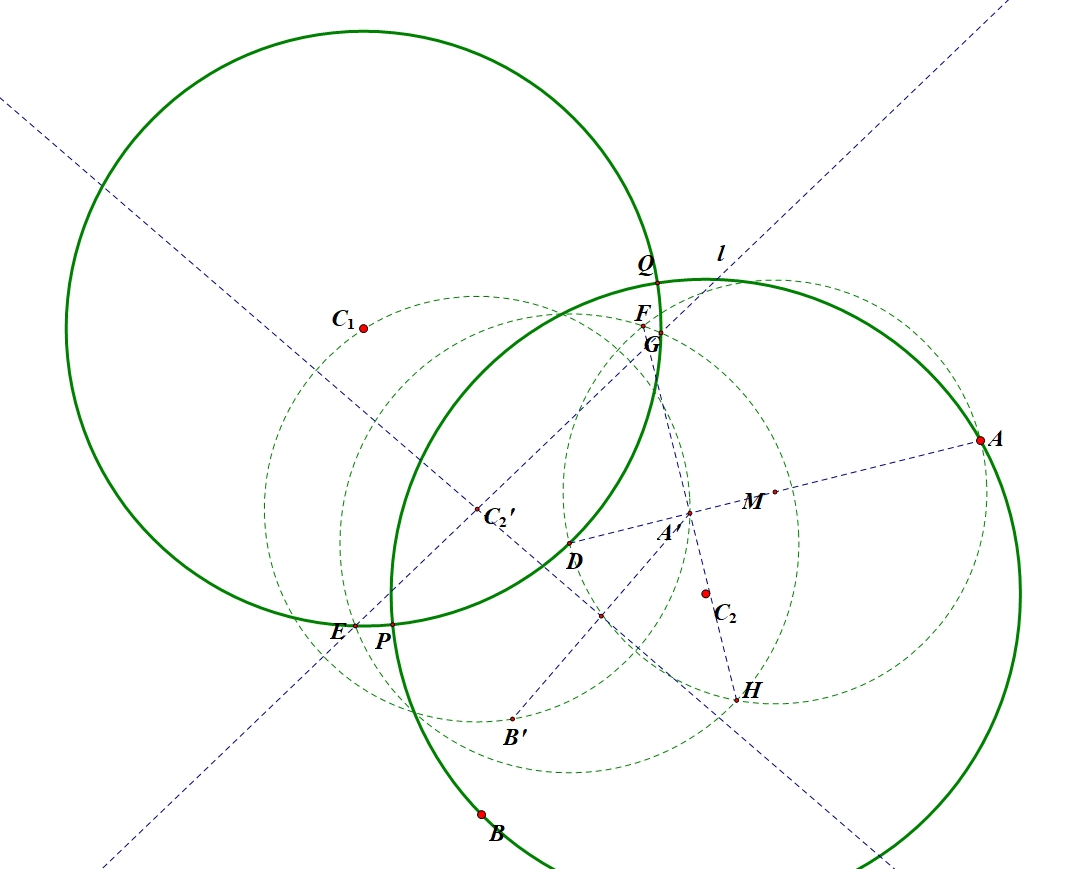
\includegraphics[scale = 0.31]{Figures/怀新一题(4).png}
        \caption{点 $A$, $B$ 均在圆外}
    \end{figure}
\end{remark}